\documentclass[tikz,border=10pt]{standalone}
\begin{document}
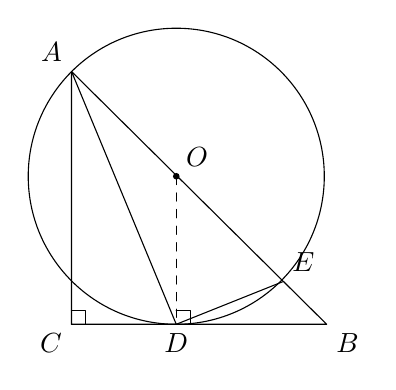
\begin{tikzpicture}[scale=1, line cap=round, line join=round]
  \coordinate (A) at (0.84,3.21);
  \coordinate (C) at (0.84,0);
  \coordinate (B) at (4.08,0);
  \coordinate (D) at (2.17,0);
  \coordinate (O) at (2.17,1.88);
  \coordinate (E) at (3.52,0.54);

  \draw (O) circle (1.88);

  \draw (A) -- (C) -- (B) -- (A);
  \draw (A) -- (D);
  \draw (D) -- (E);
  \draw[dashed] (O) -- (D);

  \draw (0.84,0) -- (1.02,0) -- (1.02,0.18) -- (0.84,0.18);
  \draw (2.17,0.18) -- (2.35,0.18) -- (2.35,0);

  \fill (O) circle (1.2pt);

  \node[above left] at (A) {$A$};
  \node[below left] at (C) {$C$};
  \node[below right] at (B) {$B$};
  \node[below] at (D) {$D$};
  \node[above right] at (E) {$E$};
  \node[above right] at (O) {$O$};
\end{tikzpicture}
\end{document}
